% Harus dimuat terlebih dahulu, digunakan agar file PDF memiliki format karakter yang benar.
% Untuk informasi lebih lanjut, lihat https://ctan.org/pkg/cmap.
\RequirePackage{cmap}

% Format dokumen sebagai paper konferensi menggunakan aturan IEEEtran terbaru (v1.8b).
% Untuk informasi lebih lanjut, lihat http://www.michaelshell.org/tex/ieeetran/.
\documentclass[conference]{IEEEtran}[2015/08/26]

% Format encoding font dan input menjadi 8-bit UTF-8.
\usepackage[T1]{fontenc}
\usepackage[utf8]{inputenc}

% Format bahasa menjadi bahasa german dan inggris.
% \usepackage[indonesian]{babel}
\usepackage[english]{babel}

% Digunakan untuk tujuan demonstrasi.
\usepackage{mwe}

% Digunakan untuk menampilkan font dengan style yang lebih baik.
\usepackage[zerostyle=b,scaled=.75]{newtxtt}

% Digunakan untuk menampilkan tabel dengan style yang lebih baik.
\usepackage{booktabs}

% Digunakan untuk menampilkan gambar pada dokumen.
\usepackage{graphicx}

% Digunakan untuk menampilkan potongan kode.
\usepackage{listings}
\lstset{
  basicstyle=\ttfamily,
  columns=fixed,
  basewidth=.5em,
  xleftmargin=0.5cm,
  captionpos=b
}

% Digunakan agar backticks (`) dapat dirender pada PDF.
% Untuk informasi lebih lanjut, lihat https://tex.stackexchange.com/a/341057/9075.
\usepackage{upquote}

% Digunakan untuk menyeimbangkan bagian akhir dokumen dengan dua kolom.
\usepackage{balance}

% Digunakan untuk menampilkan pustaka.
\usepackage[square,comma,numbers,sort&compress]{natbib}

% Mengubah format ukuran teks pada natbib.
\renewcommand{\bibfont}{\normalfont\footnotesize}

% Menambah nama penulis ketika menggunakan perintah \citet.
% Untuk informasi lebih lanjut, lihat https://tex.stackexchange.com/a/76075/9075.
\usepackage{etoolbox}
\makeatletter
\patchcmd{\NAT@test}{\else \NAT@nm}{\else \NAT@hyper@{\NAT@nm}}{}{}
\makeatother

% Digunakan untuk melakukan linewrap pada pustaka dengan url yang panjang
% jika terdapat hyphens
\usepackage[hyphens]{url}

% Digunakan untuk menambah hyperlink pada referensi.
\usepackage{hyperref}
\usepackage{longtable}

% Menonaktifkan warna dan bookmark pada hyperref.
\hypersetup{hidelinks,
  colorlinks=true,
  allcolors=black,
  pdfstartview=Fit,
  breaklinks=true
}

% Digunakan untuk membenarkan hyperref pada gambar.
\usepackage[all]{hypcap}

% Digunakan untuk menampilkan beberapa gambar
\usepackage[caption=false,font=footnotesize]{subfig}

\usepackage{stfloats}
\usepackage{float}

% Tambahkan format tanda hubung yang benar di sini
\hyphenation{
  ro-ket
  me-ngem-bang-kan
  per-hi-tu-ngan
}

\begin{document}

  % Ubah kalimat berikut sesuai dengan judul penelitian.
\title{BLOCKCHAIN-BASED NFT INTEROPERABILITY USING SMART CONTRACTS IN WEB3.0}

% Ubah kalimat-kalimat berikut sesuai dengan nama, institusi, alamat dan kontak penulis.
\author{
  \IEEEauthorblockN{Arya Abdul Azis}
  \IEEEauthorblockA{Departemen Teknik Komputer\\
    Institut Teknologi Sepuluh Nopember\\
    Surabaya, Indonesia 60111\\
    5024201069@student.its.ac.id}

  \and
  \IEEEauthorblockN{Mochamad Hariadi}
  \IEEEauthorblockA{Departemen Teknik Komputer\\
    Institut Teknologi Sepuluh Nopember\\
    Surabaya, Indonesia 60111\\
    mochar@te.its.ac.id}

  \and
  \IEEEauthorblockN{Reza Fuad Rachmadi}
  \IEEEauthorblockA{Departemen Teknik Komputer\\
    Institut Teknologi Sepuluh Nopember\\
    Surabaya, Indonesia 60111\\
    fuad@its.ac.id}
}

% Digunakan untuk menampilkan judul dan deskripsi penulis.
\maketitle

  % Mengubah keterangan `Abstract` ke bahasa indonesia.
% Hapus bagian ini untuk mengembalikan ke format awal.
\renewcommand\abstractname{Abstrak}

\begin{abstract}

  % Ubah paragraf berikut sesuai dengan abstrak dari penelitian.
  The emergence of Non-Fungible Tokens (NFTs) as a key component of the digital economy has sparked significant interest in their potential to revolutionize various industries, from art and entertainment to digital identity management. A fundamental aspect of maximizing the utility of NFTs involves ensuring their seamless operation across different blockchain platforms, which is addressed by the concept of interoperability. This thesis presents a comprehensive study and implementation of blockchain-based NFT interoperability using smart contracts within the framework of Web3.0. The research primarily focuses on developing a smart contract architecture that not only supports the standard features of NFTs but also facilitates their cross-chain interactions. By leveraging the Ethereum blockchain and utilizing the ERC-721 standard, this work establishes a robust protocol for NFT creation, transaction, and management that ensures secure, transparent, and efficient interoperability. Key aspects include the design of a decentralized application (DApp) that interacts with smart contracts to mint, manage, and transfer NFTs across blockchain boundaries. The implementation demonstrates the practicality and efficiency of the proposed system in a controlled testnet environment. Future work might explore scaling solutions, enhanced security features, and the integration of additional blockchain platforms to extend the reach and applicability of interoperable NFTs in the expanding universe of Web3.0.

\end{abstract}

% Mengubah keterangan `Index terms` ke bahasa indonesia.
% Hapus bagian ini untuk mengembalikan ke format awal.
\renewcommand\IEEEkeywordsname{Keywords}

\begin{IEEEkeywords}

  % Ubah kata-kata berikut sesuai dengan kata kunci dari penelitian.
  Non-Fungible Tokens (NFTs), Blockchain Interoperability, Smart Contracts, Web3.0, Ethereum

\end{IEEEkeywords}


  % Ubah bagian berikut sesuai dengan konten-konten yang akan dimasukkan pada dokumen
  % Ubah judul dan label berikut sesuai dengan yang diinginkan.
\section{Introduction}
\label{sec:pendahuluan}


In recent years, NFTs have come into the spotlight for both industry and academia. Data indicates that the daily transaction volume of the NFT market reaches approximately \$4.592 billion USD, while the total daily transaction volume of the crypto market is around \$341.017 billion USD. Non-Fungible Tokens (NFTs) are digital assets that represent objects like art, collectibles, and in-game items. These assets are traded over the internet, mostly with cryptocurrencies, and are typically embedded in smart contracts on a blockchain. NFTs are unique, making them non-interchangeable with similar objects, which makes them ideal for uniquely identifying something or someone. Although NFTs promise a significant impact on the current decentralized market and future business opportunities, the technology is still in its infancy. There are several challenges that need to be carefully addressed, and many significant opportunities that need to be seized.

NFTs, backed by blockchain technology and smart contracts, offer tremendous opportunities for the creative industry, though their presence has disrupted the market. However, NFTs also have limitations stemming from the underlying blockchain technology. Blockchain itself ensures trust within its distributed system by relying on computers (often called "miners") to solve complex mathematical problems. One major challenge in the evolution of blockchain technology is interoperability. Although blockchains provide robust and reliable solutions, the various types and variants of blockchains currently in existence often struggle to interact and communicate effectively. This implies that smart contracts or NFTs developed on one blockchain may not be compatible or recognized by another type of blockchain. This limitation restricts the blockchain's ability to grow and integrate with larger industry systems, such as finance, healthcare, or international business.

Blockchain and Smart Contracts are crucial foundations in realizing the vision of Web3.0. Blockchain provides transparency, security, and trust by storing data on a decentralized network, while Smart Contracts enable the automation of transactions and agreements in the digital world without intermediaries. The combination of these technologies could lay the foundation for a new era in the digital world, where interactions are more secure, transparent, and seamless.

The discussion in this paper begins with a presentation on other research (Section \ref{sec:penelitianterkait}). It then continues with an explanation of the architecture of the system developed (Section \ref{sec:arsitektur}). Based on this, we show the results of testing and analysis (Section \ref{sec:hasil}). Finally, conclusions from the research conducted are presented (Section \ref{sec:kesimpulan}).








  % Ubah judul dan label berikut sesuai dengan yang diinginkan.
\section{Related Research}
\label{sec:penelitianterkait}

% Ubah paragraf-paragraf pada bagian ini sesuai dengan yang diinginkan.


Several other studies have been conducted, as formulated by \citet{Wang2021}, which suggest that NFTs can transform the digital or virtual asset market. The results of this research provide an in-depth understanding of NFT technology, its potential, and the challenges it faces. Additionally, research results from \citet{Zheng2020} have yielded knowledge in the form of a review on the latest smart contract technology, challenges in various aspects of creation, deployment, execution, and resolution of smart contracts, comparisons of several major smart contract platforms, and reviews on smart contract and blockchain technology. Cited from research previously written by \citet{Malik2023}, the study examines blockchain technology's impact on the creative industries, such as music, graphic design, gaming, and software. In this journal, they highlight how NFTs (non-fungible tokens) and smart contracts offer exciting opportunities for the creative industry. Although this technology has created significant excitement in the market, amidst the hype, real value emerges for the industry. Traditionally, creators in the creative industry often had to rely on powerful intermediaries to distribute and monetize their creations. However, with the advent of NFTs and smart contracts, creators can now be closer to their consumers/buyers of content. Additionally, this journal also explores the market share and "transaction costs" creators face when distributing their creative content and how smart contracts and NFTs can change market dynamics by reducing these costs.
  % Ubah judul dan label berikut sesuai dengan yang diinginkan.
\section{ARCHITECTURE}
\label{sec:arsitektur}

\subsection{Arsitektur Sistem}
\begin{figure}[H] \centering
  % Nama dari file gambar yang diinputkan
  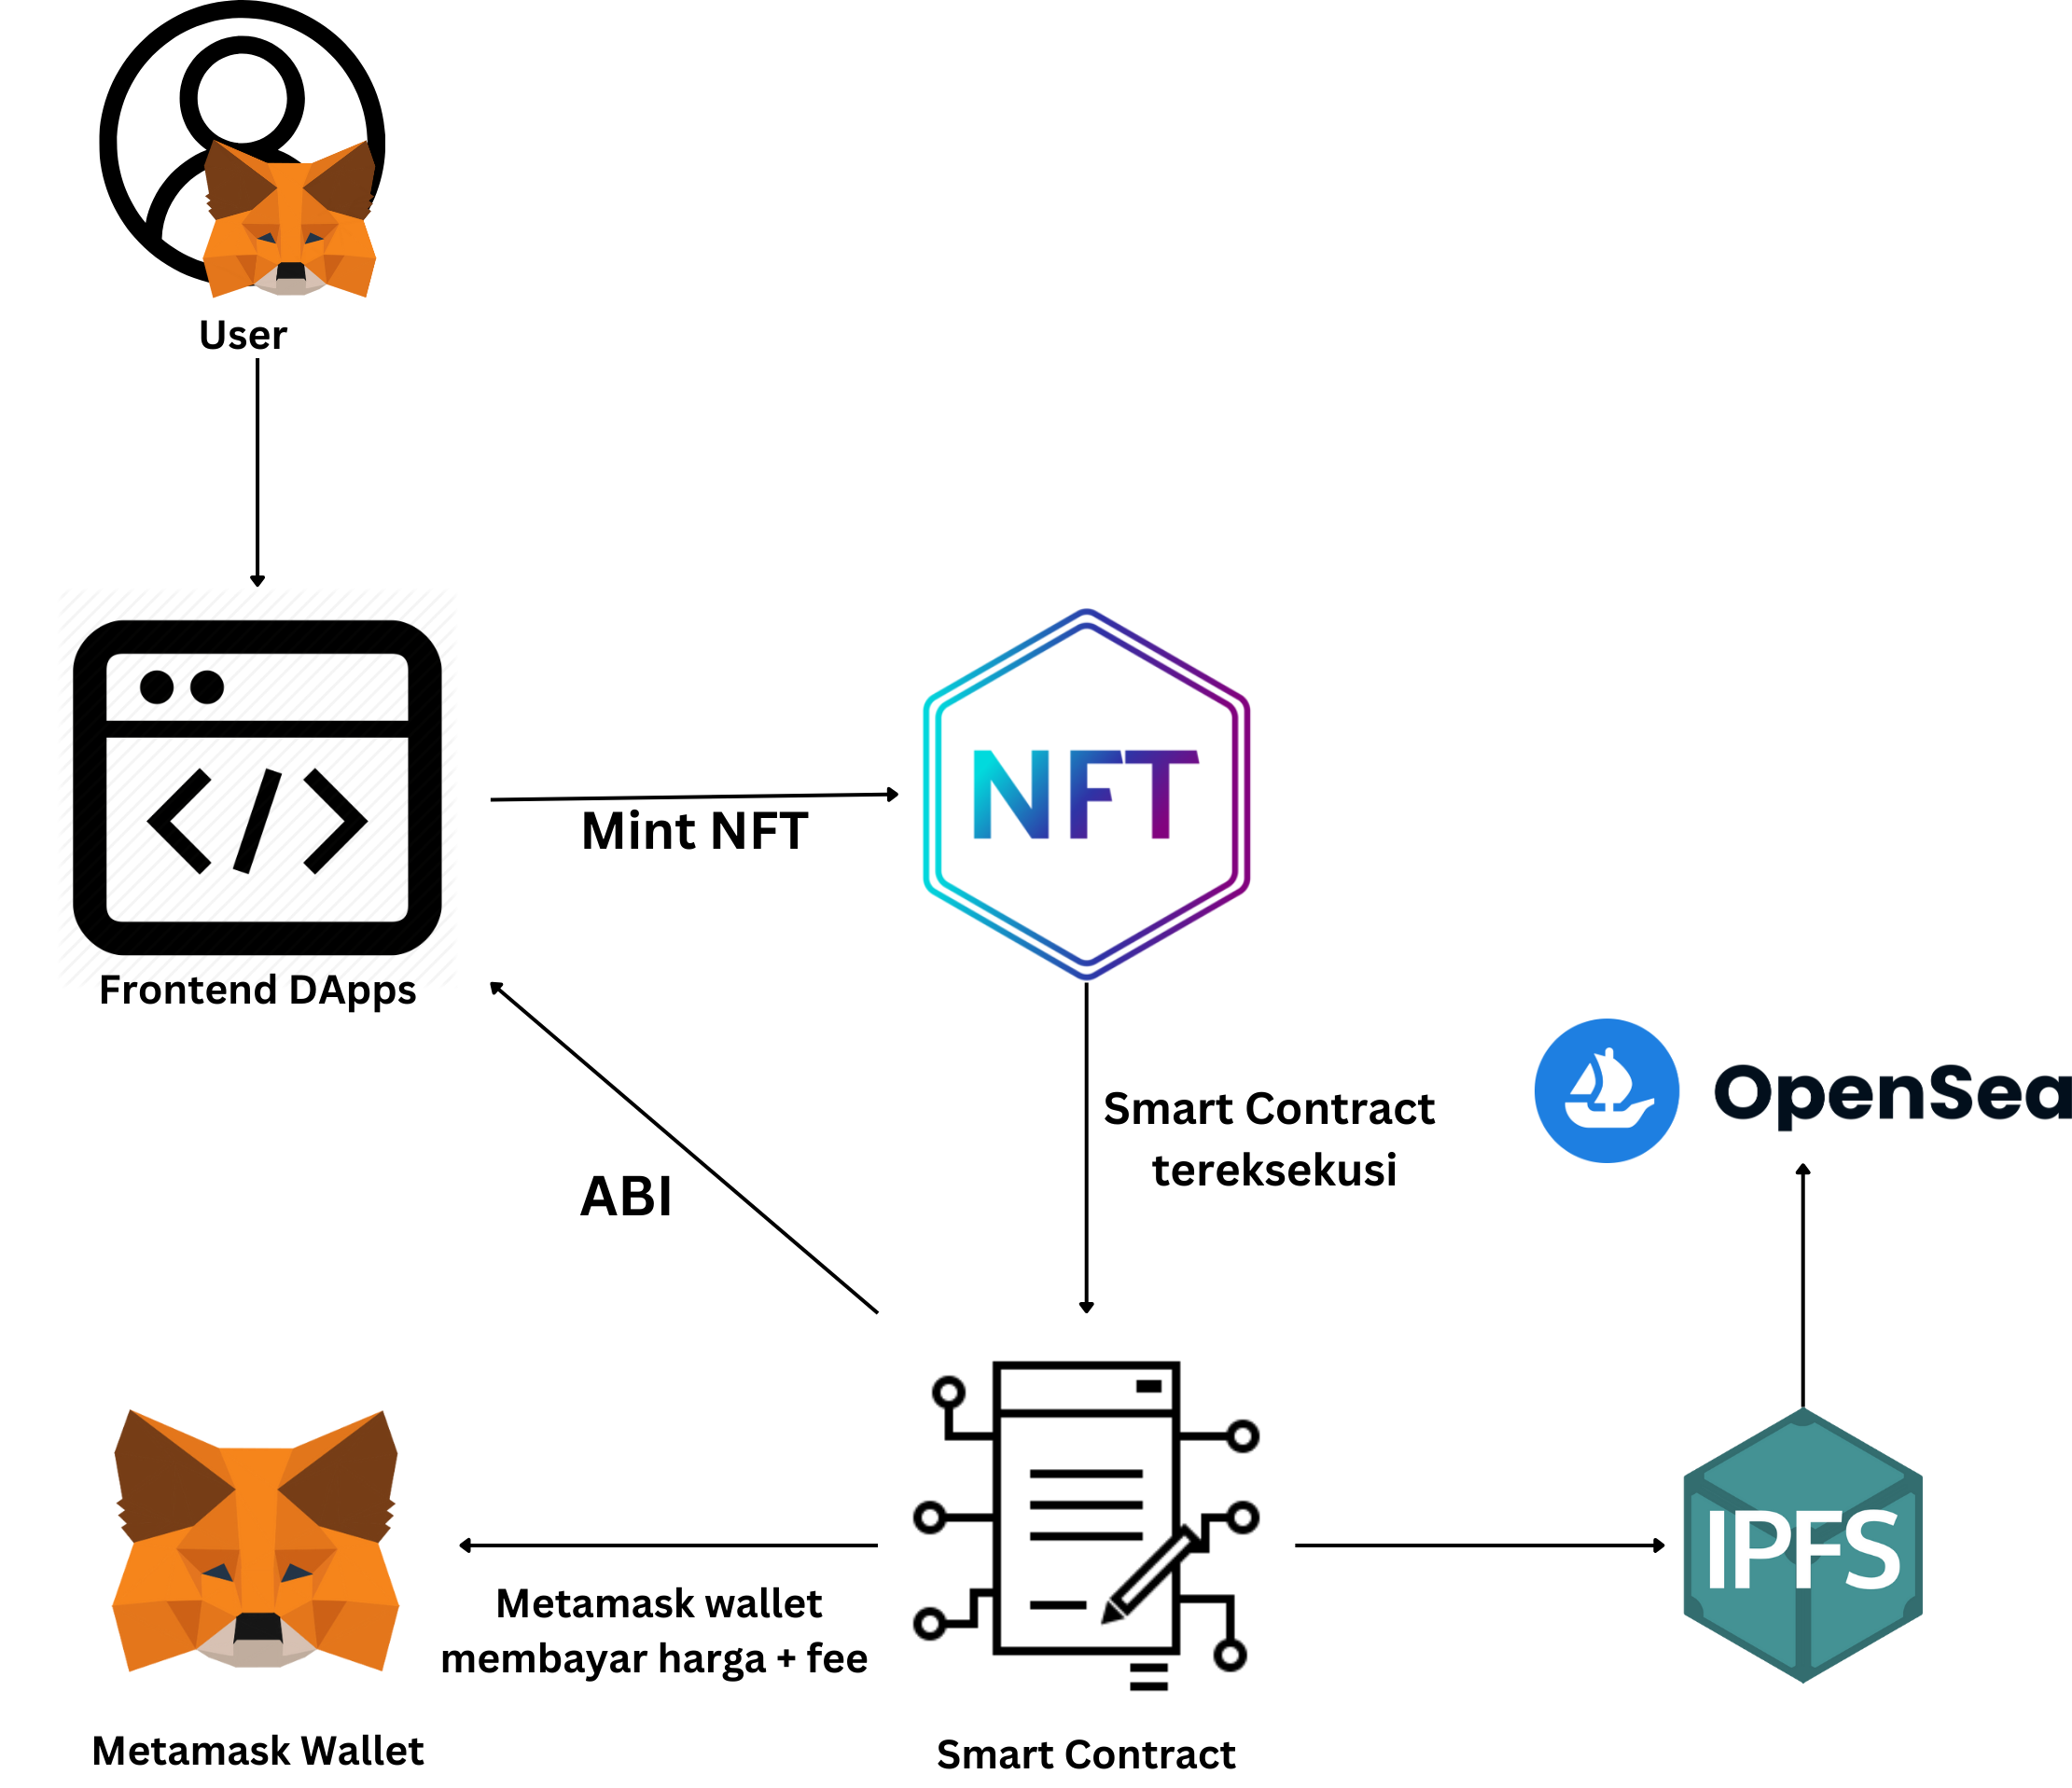
\includegraphics[scale=0.14]{gambar/desain_sistem_new.png}
  % Keterangan gambar yang diinputkan
  \caption{Desain sistem}
  % Label referensi dari gambar yang diinputkan
  \label{fig:desain_sistem}
\end{figure}

In the development of this smart contract system to function as intended by the author for completing this thesis, the author has designed a system architecture. In this system architecture, there is a role for the user who can become the owner of a token, and the user is the party with limited access to a token within a specified time. There is also a front end for the minting process of NFT tokens. To access the front end, both the owner and the user must connect using a Metamask wallet to interact.

On the front end, it connects with the smart contract when a user performs Minting, where the process involves the user uploading a digital asset they own to IPFS through a backend application, which then returns a Content Identifier (CID). A CID is a file address within IPFS used to access that file. The obtained CID is then uploaded to the blockchain network and becomes a token. Data about the available NFTs can be directly accessed by the front end through the smart contract on the blockchain.

% \vspace{0.5 cm}

\subsection{Proses Minting}
\begin{figure}[H] \centering
  % Nama dari file gambar yang diinputkan
  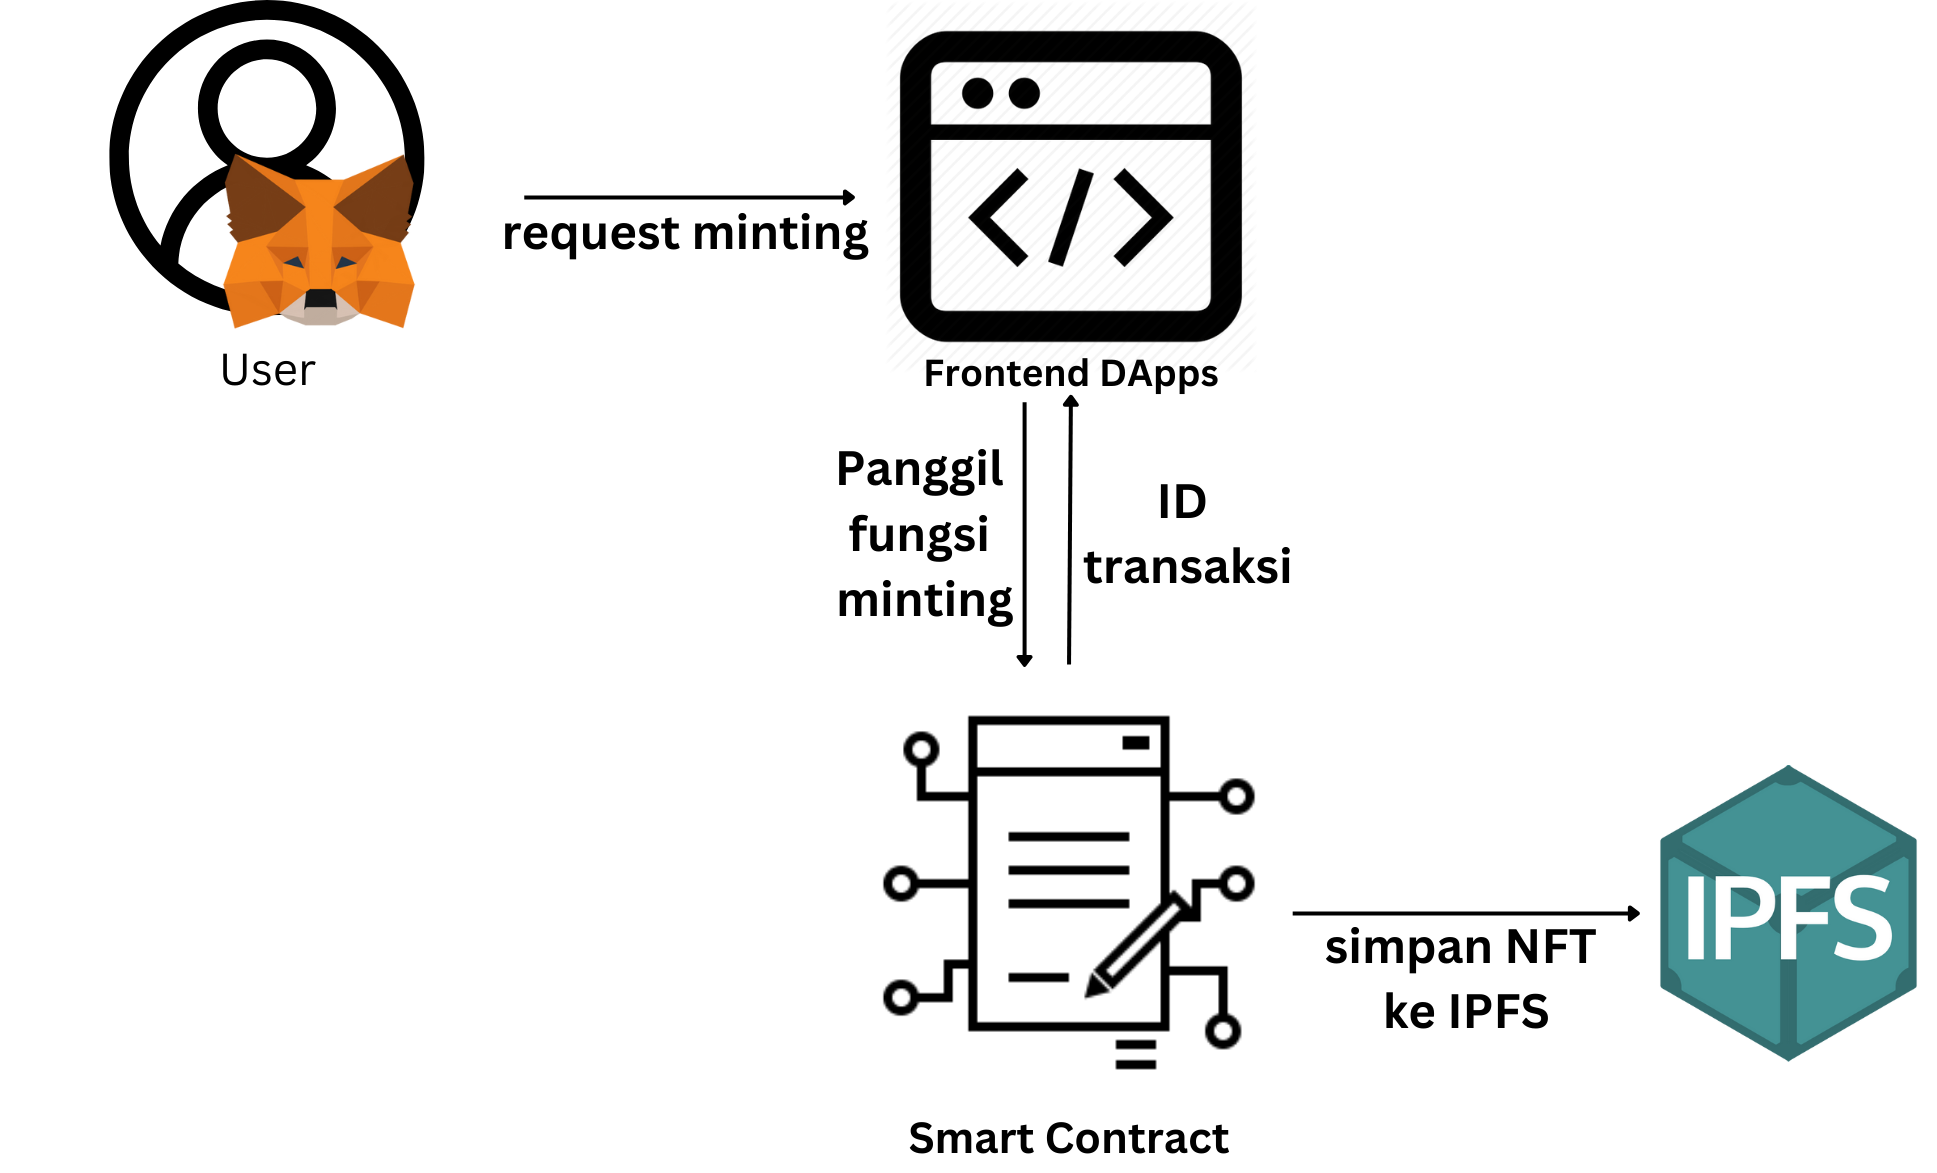
\includegraphics[scale=0.17]{gambar/proses_minting.png}
  % Keterangan gambar yang diinputkan
  \caption{Desain sistem}
  % Label referensi dari gambar yang diinputkan
  \label{fig:proses_minting}
\end{figure}

The minting process is the initial step where a new NFT is created on a platform. During this process, various important details about the NFT must be defined, including its name, description, category, available supply, and the visual asset representing the NFT, which could be a 2D image, 3D model, or video. The initial price, the collection that includes the NFT, and other attributes must also be determined. Once the minting process is complete, the data from the newly created NFT is stored in the InterPlanetary File System (IPFS), which allows for decentralized storage and access to data. This storage ensures that all related information, such as ownership recorded in the NFT’s attributes, can be accessed permanently and securely.

\subsection{Metode Yang Digunakan}
\begin{figure}[H] \centering
  % Nama dari file gambar yang diinputkan
  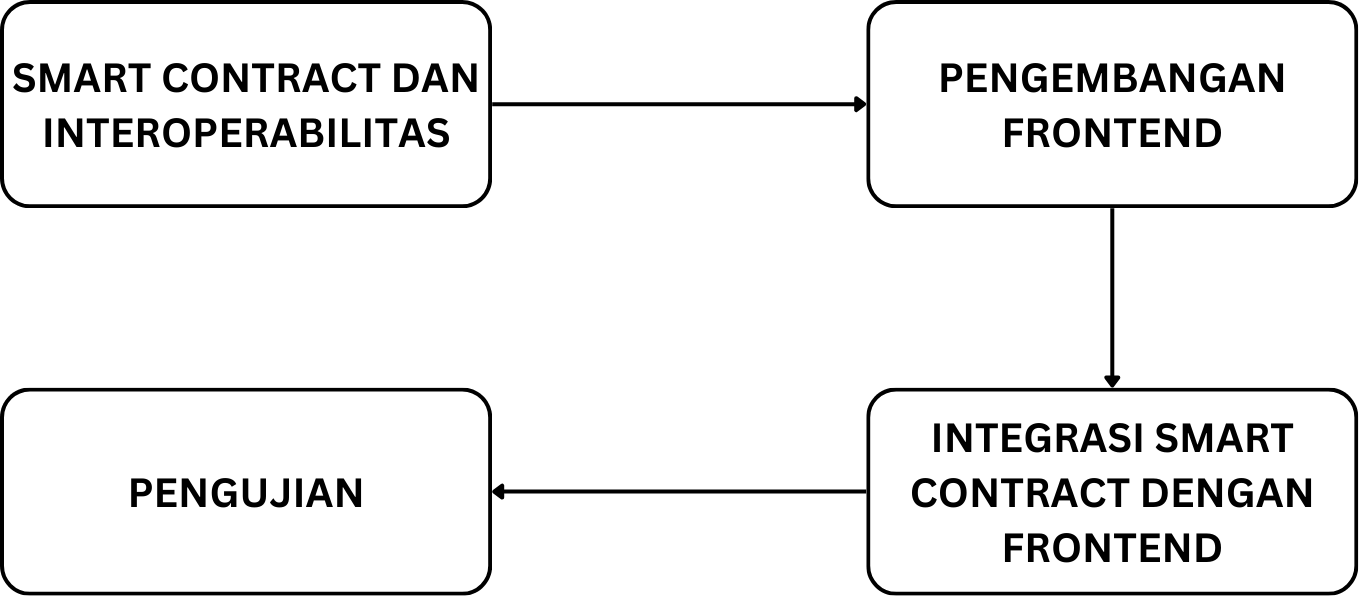
\includegraphics[scale=0.20]{gambar/metodologi_new.png}
  % Keterangan gambar yang diinputkan
  \caption{Metodologi Pengerjaan}
  % Label referensi dari gambar yang diinputkan
  \label{fig:metodologi}
\end{figure}

\subsubsection{Smart Contract dan Interoperabilitas}
In this stage, the author develops a smart contract system used for creating interoperable tokens using the Solidity programming language. This smart contract system acts as a bridge to process requests generated from user interactions on the frontend to the blockchain network. Upon compiling the smart contract, an Application Binary Interface (ABI) is generated, which can be used on the frontend for encoding and decoding data, allowing the frontend application to send precise instructions to the smart contract and understand the data returned by it. The smart contract developed by the author includes several core functions for the developed token.

\subsubsection{Pengembangan Frontend} 
To integrate a React application with the Ethereum blockchain, we utilize two primary libraries: ethers.js and web3.js. These libraries provide the necessary functionality to interact with the Ethereum blockchain, though they approach it slightly differently. Ethers.js is known for its minimalistic API and ease of use, which is particularly suitable for projects with simpler needs and a focus on reading and writing data to the blockchain. This library offers powerful functions for interacting with smart contracts, such as sending transactions, reading contract statuses, and handling event notifications.

\subsubsection{Integrasi Smart Contract dengan Frontend}
This stage enables applications built with React.js to interact directly with smart contracts deployed on the Ethereum network. To achieve this integration, we use the ethers.js library, which provides a clean and user-friendly interface for communicating with Ethereum.

Once the smart contract is developed and deployed, the ABI (Application Binary Interface) of the contract is used to construct a contract instance within the React application. The ABI allows the frontend to understand what functions are available in the smart contract, including the variables and data types used. With this information, ethers.js can invoke these functions, such as safeMint or transferOwnership, according to the logic defined in the contract.

\subsubsection{Pengujian}
This stage includes several steps for testing the smart contract, namely unit testing and integration testing.

\begin{itemize}
    \item Unit Testing
    This testing focuses on validating each component individually. In the context of a React.js frontend, this means testing components separately to ensure that they behave as expected. Unit testing is also conducted on the smart contract functions to verify their business logic, such as minting or token transfer functions. This testing is typically performed using the React framework for frontend and Hardhat for smart contracts.

    \item Integration Testing
    Following unit testing, the next step is integration testing, which ensures that all components in the application work well when combined. In the context of smart contract integration, this involves testing the interaction between the React.js frontend and the smart contract through ethers.js or web3.js. Integration testing helps detect issues in the data flow between the frontend and blockchain, including transaction validation and correct state updates.
    
\end{itemize}
  % Change the title and label as desired.
\section{RESULTS}
\label{sec:results}
\subsection{Results}
The overall result of the developed system is a web interface, Non-Fungible Token (NFT), and interoperable smart contract. The following sections detail each result of the developed system.

\subsubsection{Web Interface}
The initial web interface displays a list of NFT collections that are available for minting. The NFT can initially be owned by the address that mints it first, and ownership can be transferred to another address. At the initial dashboard, users must press the \emph{Connect Wallet} button, which will then connect to the Metamask Wallet account. From this connection, users obtain an address that can be used to mint NFT tokens. This intuitive interface simplifies the process of connecting to the blockchain, ensuring that even users new to the world of NFTs can easily navigate and understand the steps involved in acquiring and managing digital assets. Moreover, the dashboard is designed to be user-friendly, providing clear and concise information, which aids in fostering a seamless interaction between the user and the blockchain technology.

\begin{figure}[H] \centering
  % Name of the image file
  \frame{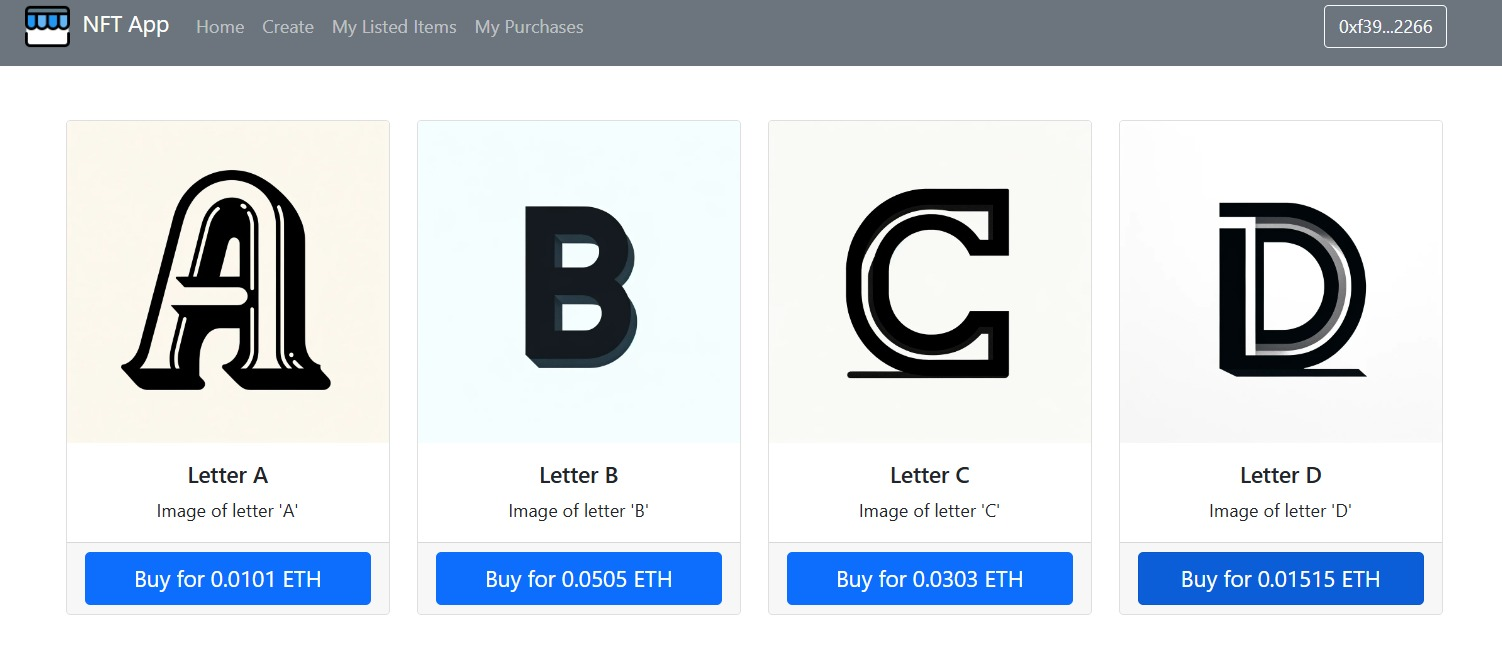
\includegraphics[scale=0.17]{gambar/tampilan_aplikasi.jpeg}}
  % Caption for the image
  \caption{View of the web interface}
  % Reference label for the image
  \label{fig:web_view}
\end{figure}

\begin{figure} [H] \centering
  % Nama dari file gambar yang diinputkan
  \frame{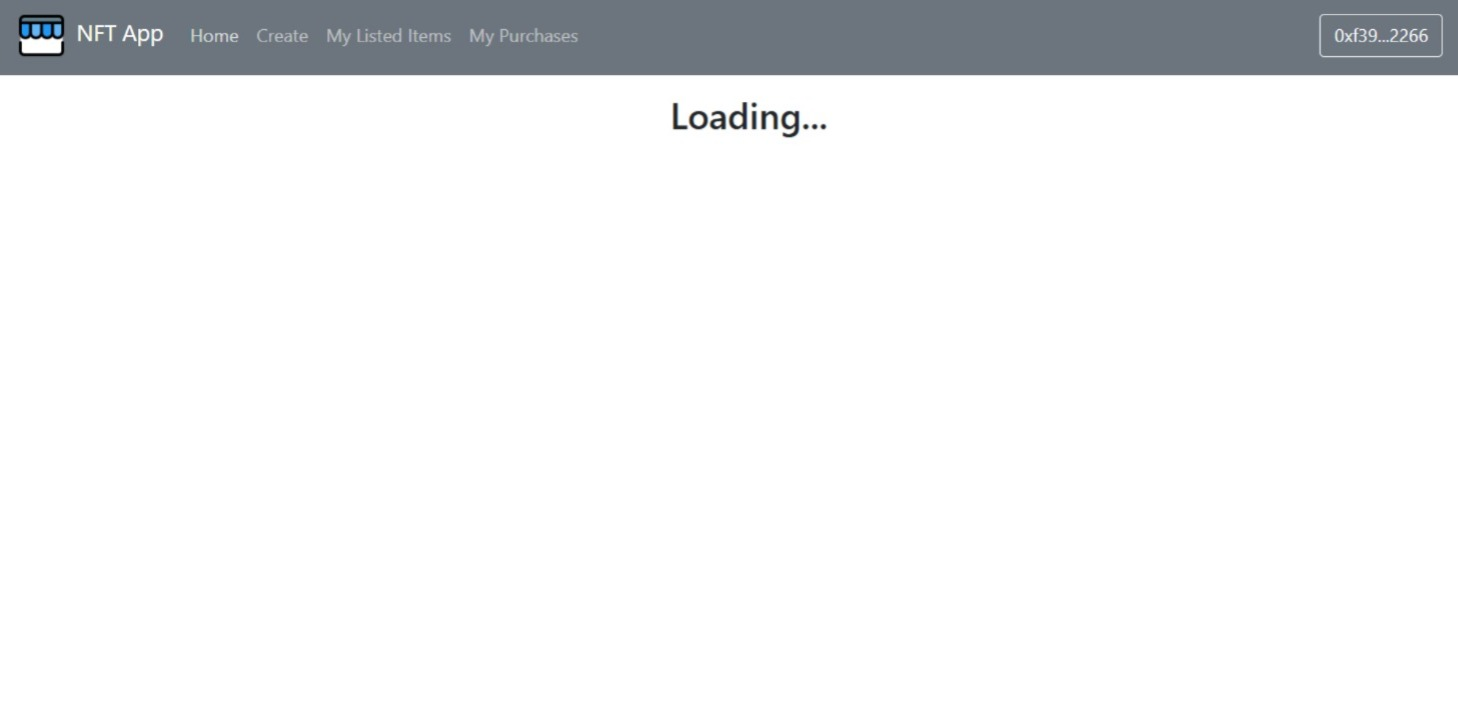
\includegraphics[scale=0.17]{gambar/home_page.jpg}}
  % Keterangan gambar yang diinputkan
  \caption{View of the first appearance of the web}
  % Label referensi dari gambar yang diinputkan
  \label{fig:homepage}
  \end{figure}

  In the image referred to as \ref{fig:homepage}, the initial homepage view is presented when users click the home button on the top navigation bar. This website features several pages accessible through the navigation bar, such as Home, Create, My Listed Items, and My Purchases. These interfaces become available once the user has successfully connected the web to the Metamask Wallet, evidenced by the display of the Metamask Wallet address on the upper right of the navigation bar. On this initial screen, users can view NFTs that have been uploaded for purchase or minting. However, if no NFTs have been uploaded yet, the display will only show the message "\emph{Loading...}".
   
  \begin{figure} [H] \centering
    % Nama dari file gambar yang diinputkan
    \frame{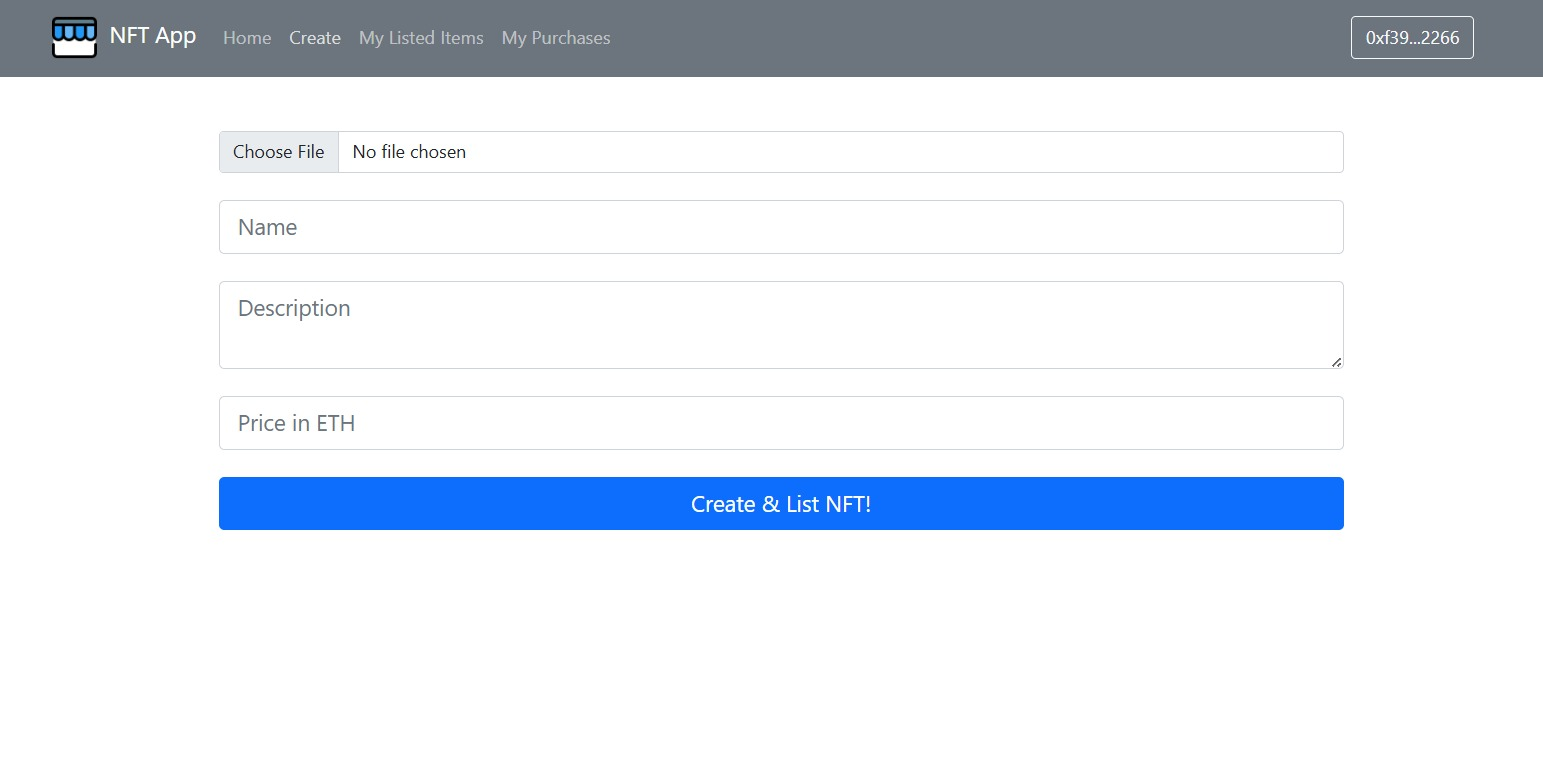
\includegraphics[scale=0.15]{gambar/create_page.jpeg}}
    % Keterangan gambar yang diinputkan
    \caption{View of the create page}
    % Label referensi dari gambar yang diinputkan
    \label{fig:createpage}
    \end{figure}

    In the image referred to as \ref{fig:createpage}, the create page is displayed. This page allows users to upload an NFT in the form of an image to the website. Once uploaded, the NFT will appear on both the home page and the my listed items page. Additionally, any NFT uploaded here will also be directly available for other users to view and interact with, enhancing the visibility and accessibility of newly minted NFTs within the platform. This integration ensures that NFT creators can immediately showcase their digital assets to potential buyers, facilitating a seamless transition from creation to sale.

  \begin{figure} [H] \centering
    % Nama dari file gambar yang diinputkan
    \frame{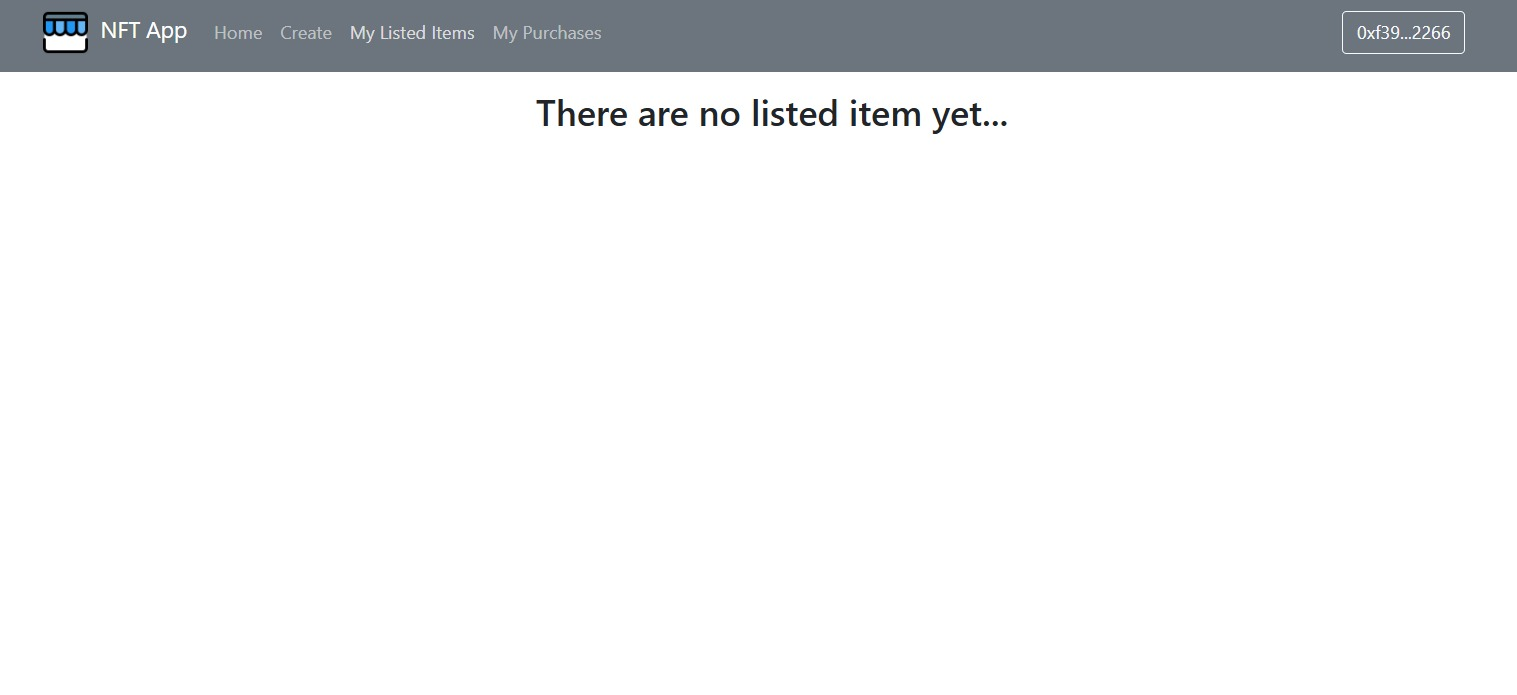
\includegraphics[scale=0.15]{gambar/listing_page.jpg}}
    % Keterangan gambar yang diinputkan
    \caption{View of the my listed item page}
    % Label referensi dari gambar yang diinputkan
    \label{fig:listingpage}
    \end{figure}
  
    In the image referenced as \ref{fig:listingpage}, the my listed items page is shown. This page allows users to view the NFTs they have uploaded when they used the create function. However, if no NFTs have been uploaded yet, the page will display the message "\emph{There are no listed items yet}". This setup ensures that users can easily track and manage their digital assets directly from their dashboard once they have engaged in creating and listing new NFTs.    

  \begin{figure} [H] \centering
    % Nama dari file gambar yang diinputkan
    \frame{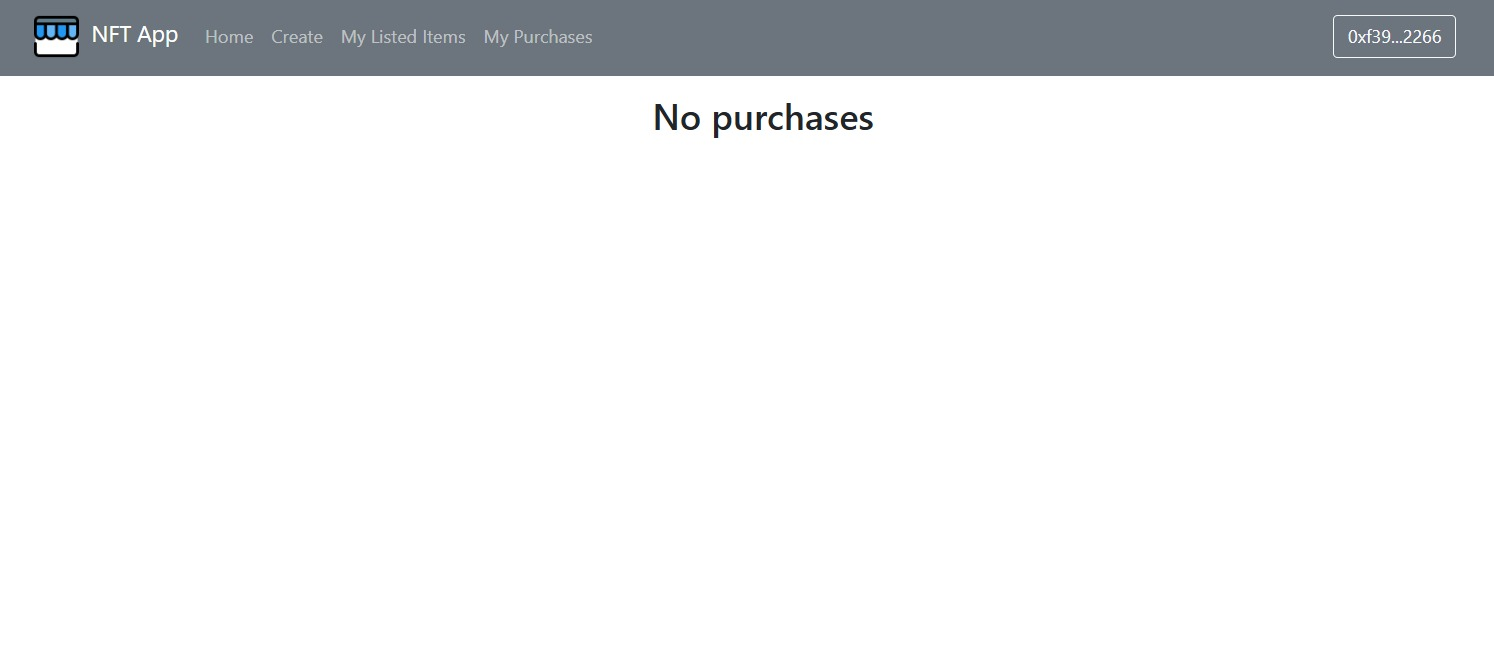
\includegraphics[scale=0.15]{gambar/purchase_page.jpg}}
    % Keterangan gambar yang diinputkan
    \caption{View of the my purchases page}
    % Label referensi dari gambar yang diinputkan
    \label{fig:purchasepage}
    \end{figure}
  
    In the image referenced as \ref{fig:purchasepage}, the display of the my purchase page is shown. This page is designed specifically to allow users to view all NFTs they have acquired through purchases on the main page of the platform. Once a purchase is made, the NFTs are listed on this page, providing a visual display and details of each NFT owned. Additionally, this page offers a transfer ownership function, which enables the owner to transfer the ownership of an NFT to another user with a different address. This feature is crucial for supporting flexibility and liquidity in NFT trading in the market. However, if the user has not made any purchases, the page will display the message "\emph{No purchases}", indicating that there are no NFTs available to display or transfer.

\subsubsection{Smart Contract}
In the development of blockchain-based applications, integrating the smart contract with user interfaces such as React.js becomes crucial. The smart contract built using Solidity can be deployed on Ethereum testnets, such as the Sepolia Testnet, which provides an environment similar to the Ethereum mainnet but without requiring high transaction fees.

The deployment process is carried out where the smart contract will be deployed to several blockchain networks, but for this testing, only the Sepolia testnet is used. During the deployment process, a gas or fee will be charged, which can be paid using Ethereum in the Metamask wallet. Details of this transaction can be seen on Etherscan.

\begin{figure} [H] \centering
  % Name of the image file
  \frame{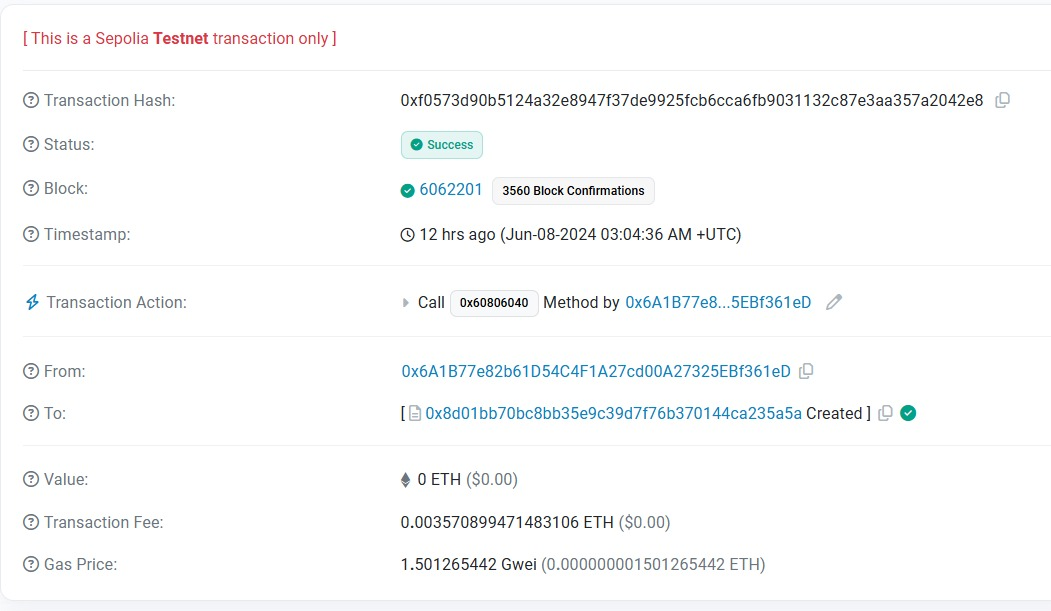
\includegraphics[scale=0.24]{gambar/etherscan.jpeg}}
  % Caption for the image
  \caption{Transaction details on Etherscan}
  % Reference label for the image
  \label{fig:transaction}
\end{figure}

\subsubsection{Non-Fungible Token (NFT)}
Non-Fungible Tokens (NFT) also undergo several stages before they can be stored in The Interplanetary File System (IPFS) and then be published on OpenSea test net. In this thesis work, Pinata is used as a platform to upload NFT photos and JavaScript Object Notation (JSON) data so that it can be minted as a Uniform Resource Identifier (URI) on the smart contract. This is necessary so that the minted NFT has an image that can be viewed on OpenSea.

\begin{figure} [H] \centering
  % Name of the image file
  \frame{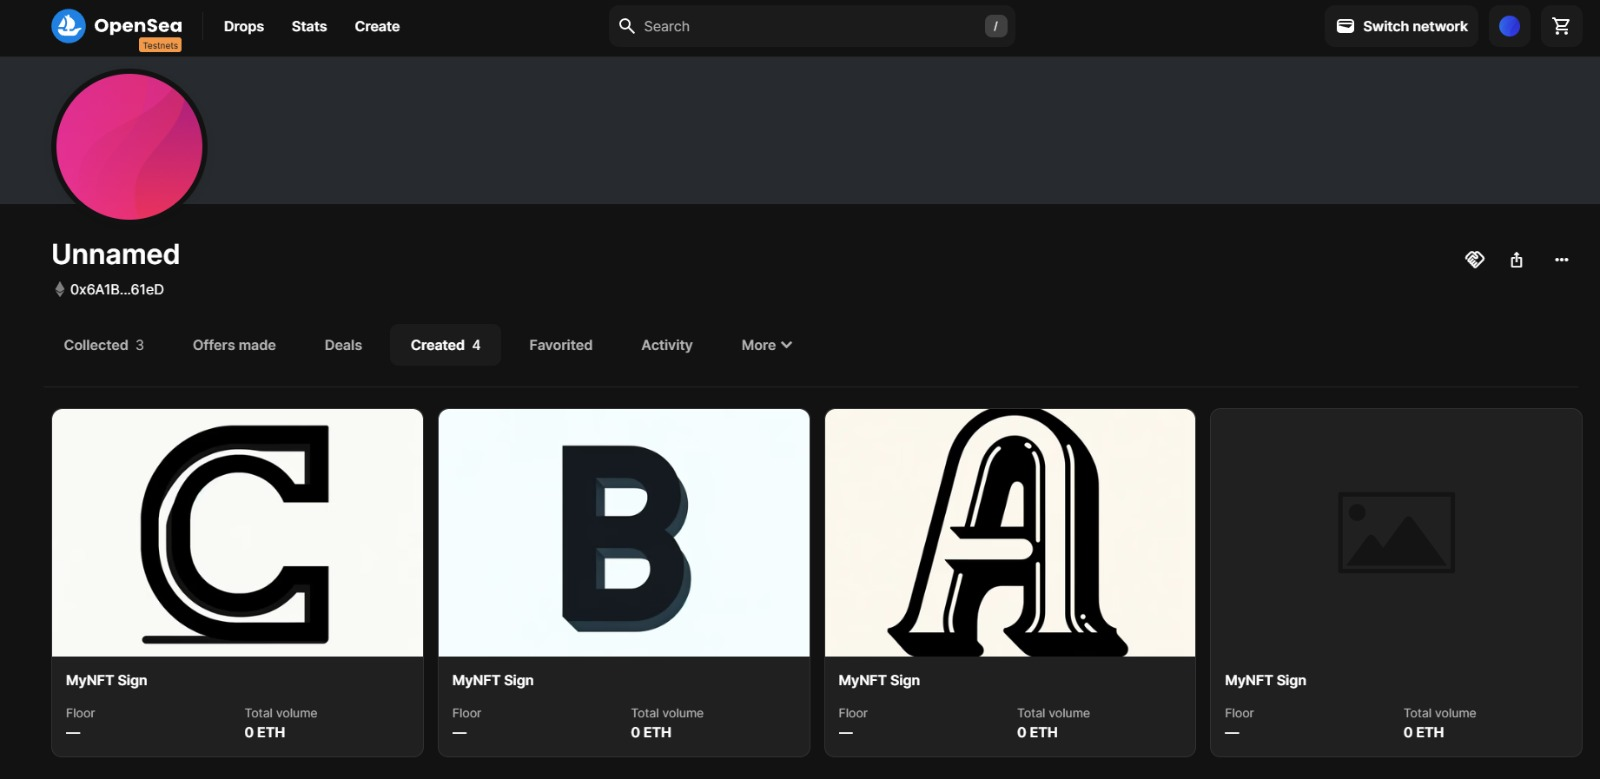
\includegraphics[scale=0.15]{gambar/opensea.jpeg}}
  % Caption for the image
  \caption{NFT uploaded on Opensea}
  % Reference label for the image
  \label{fig:opensea}
\end{figure}

\subsection{Testing Features of Smart Contract Interoperability}
The testing expectations from the smart contract system include the following:
\begin{itemize}
    \item Users can mint NFT tokens, after which the ownership of these NFTs can be viewed on the test net platform OpenSea.

    \item Users from different Networks can communicate with each other, and the ownership of the NFT tokens can move from user A on network A' to user B on network B'.
\end{itemize}

Here is the data regarding the wallet used in testing:

\begin{table}[htbp]
  \centering
  \caption{Account detail for smart contract testing}
  \label{tab:volume}
  \scalebox{1.2}{
    \begin{tabular}{|c|p{2cm}|p{2cm}|}
      \hline
      \textbf{Account} & \textbf{Address} & \textbf{Network}
      \\
      \hline
      A & 0x6A1B77e \newline 82b61D54C4 \newline F1A27cd00A27 \newline 325EBf361eD & Sepolia \newline Ethereum \newline Testnet
      \\ 
      \hline
      B & 0xD066d6576 \newline D9485Eb2
      \newline c2a41BB8B52EcE \newline 17a0557d6 & BNB \newline Chain \newline Testnet \\
      \hline
      \end{tabular}    
  }
\end{table}

The following are the steps of testing the smart contract system that will be conducted:

\begin{itemize}
    \item User A will mint an NFT first

    \begin{figure} [H] \centering
    % Name of the image file
    \frame{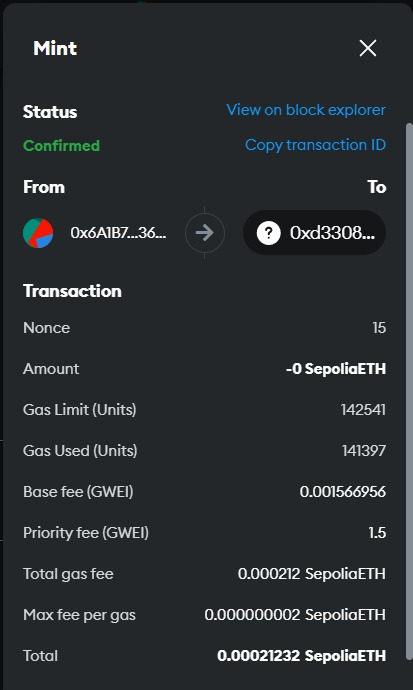
\includegraphics[scale=0.23]{gambar/riwayat_transaksi.jpeg}}
    % Caption for the image
    \caption{Minting transaction history on Metamask Wallet}
    % Reference label for the image
    \label{fig:minting}
    \end{figure}

    \item The details on Etherscan can also be seen in the image below, showing details like the transaction hash, block, and the type of token, which is ERC-721.

    \begin{figure} [H] \centering
    % Name of the image file
    \frame{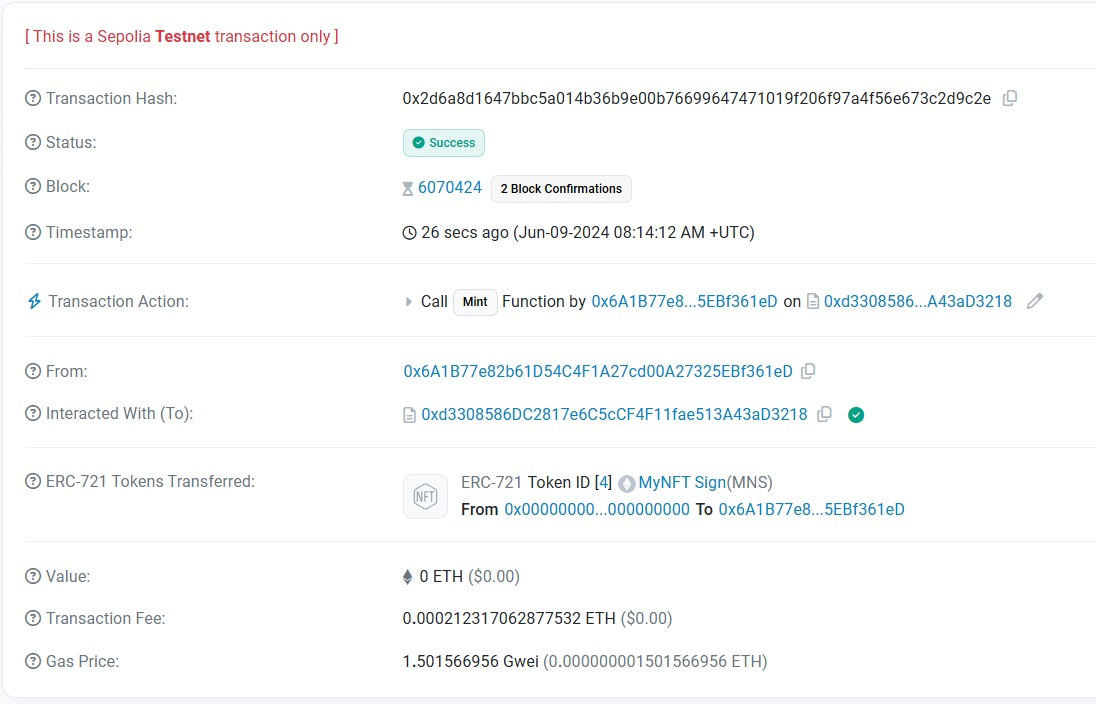
\includegraphics[scale=0.2]{gambar/detail_transaksi_etherscan.jpeg}}
    % Caption for the image
    \caption{Transaction details on Etherscan}
    % Reference label for the image
    \label{fig:detail_transaction_etherscan}
    \end{figure}

    \item Then, on Etherscan, the details of the NFT that has been minted can be seen as in the following image

    \begin{figure} [H] \centering
    % Name of the image file
    \frame{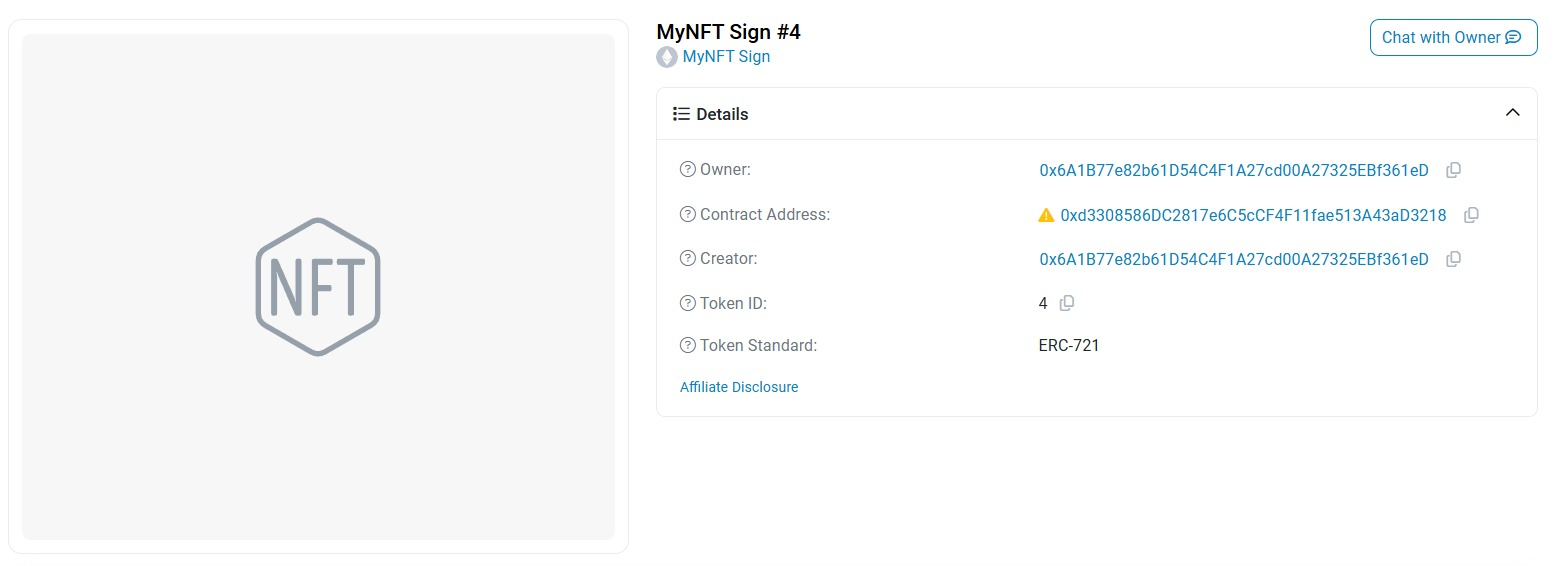
\includegraphics[scale=0.165]{gambar/detail_nft_etherscan.jpeg}}
    % Caption for the image
    \caption{NFT Details on Etherscan}
    % Reference label for the image
    \label{fig:detail_nft_etherscan}
    \end{figure}

    \item After the process is successful, the NFT that has been minted can be seen on the platform OpenSea. In this test case, the minted NFT is "Letter D".

    \begin{figure} [H] \centering
    % Name of the image file
    \frame{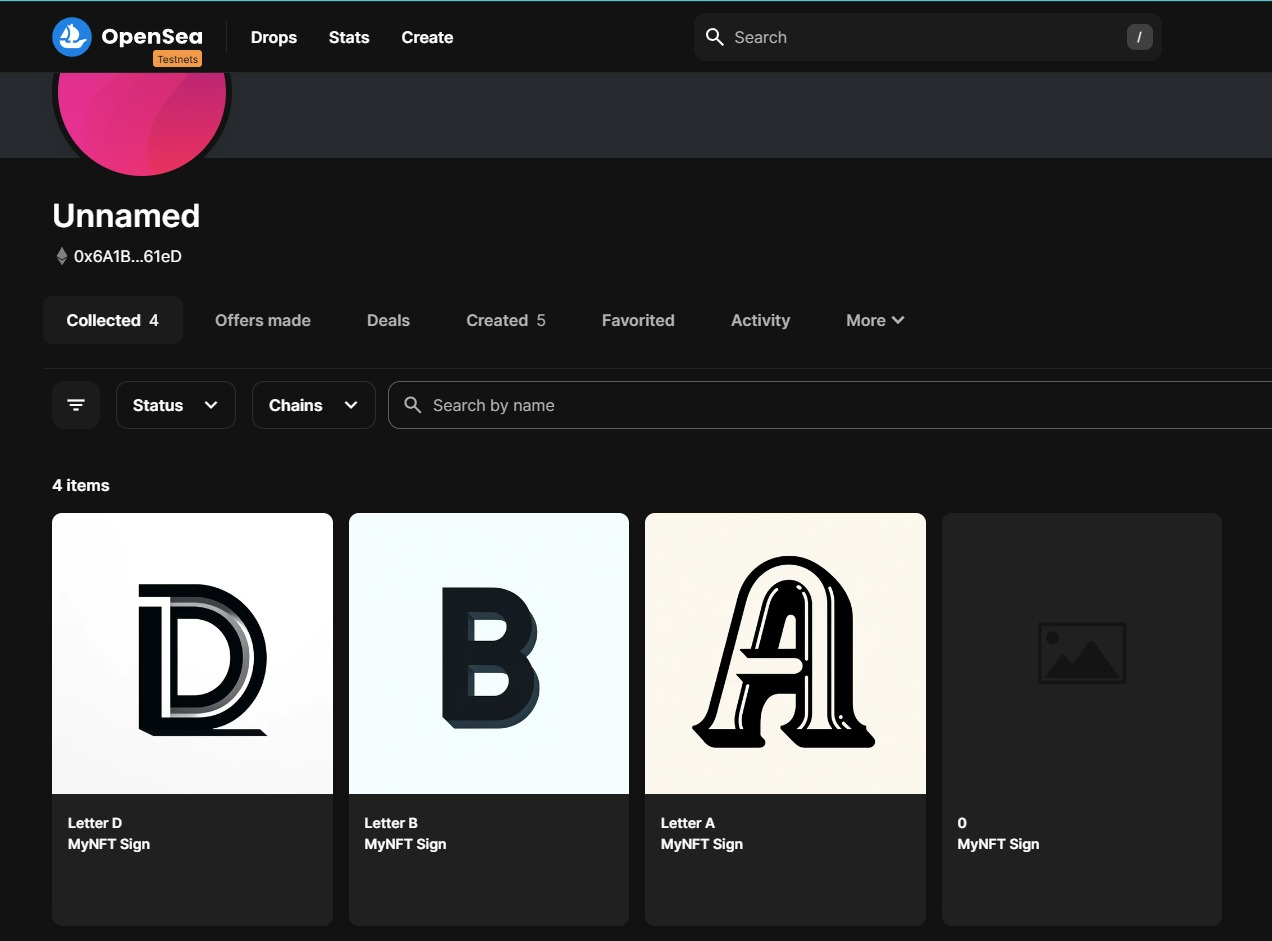
\includegraphics[scale=0.15]{gambar/nft_pada_opensea.jpeg}}
    % Caption for the image
    \caption{NFT on OpenSea}
    % Reference label for the image
    \label{fig:nft_opensea}
    \end{figure}

    \item After the NFT is created, the next step is to lock the NFT to be sent to user B on network B'. The function of locking is to ensure that the token data is not changed during the transfer process, maintaining the trust and authenticity of the NFT data. It is also useful to signal to all related parties (users, smart contracts on other networks) that the token is undergoing a transfer process, and operations on the token should be suspended until the process is completed.

    \begin{figure} [H] \centering
    % Name of the image file
    \frame{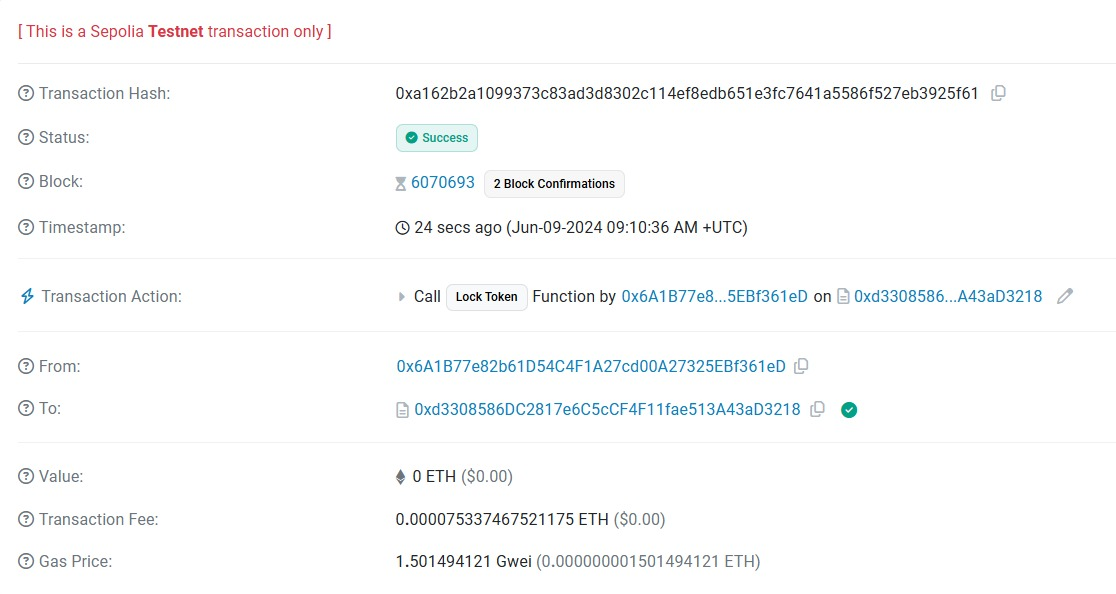
\includegraphics[scale=0.2]{gambar/lock_token.jpeg}}
    % Caption for the image
    \caption{Lock Token function details on Etherscan}
    % Reference label for the image
    \label{fig:locktoken}
    \end{figure}

    \item After completing the lock token process, then the bridge transfer function can be executed. This function facilitates the secure transfer of NFTs between blockchains by ensuring that the NFT is locked during the transfer process and providing transparent visibility of the transfer event through recorded events. This is a key component in building interoperable applications that allow digital assets to move across blockchain ecosystems.

    \begin{figure} [H] \centering
    % Name of the image file
    \frame{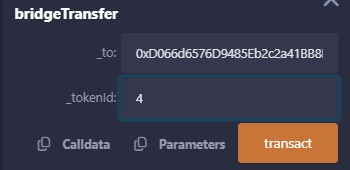
\includegraphics[scale=0.5  ]{gambar/bridge_transfer.jpeg}}
    % Caption for the image
    \caption{Bridge transfer parameters}
    % Reference label for the image
    \label{fig:bridge_transfer}
    \end{figure}

    \item In the image \ref{fig:bridge_transfer}, there are two parameters: "\texttt{"\_to"}", used to receive the parameter address of user B, and "\texttt{"\_tokenId"}" to receive arguments from the NFT token. After the transaction is executed, it will be followed by payment on the Metamask Wallet.

    \begin{figure} [H] \centering
    % Name of the image file
    \frame{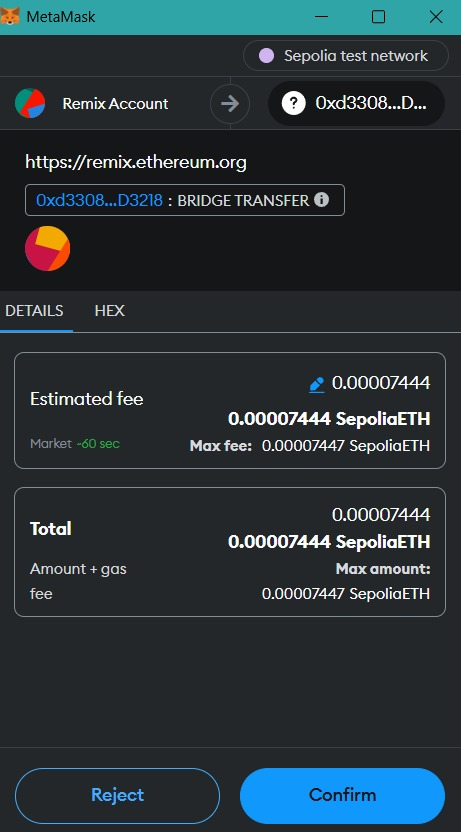
\includegraphics[scale=0.2]{gambar/verifikasi_metamask_wallet.jpeg}}
    % Caption for the image
    \caption{Payment on Metamask Wallet}
    % Reference label for the image
    \label{fig:metamask_payment}
    \end{figure}

    \item After the transaction is successful, the record of the transaction is stored on the blockchain and can be viewed on Etherscan as shown in the image below.

    \begin{figure} [H] \centering
    % Name of the image file
    \frame{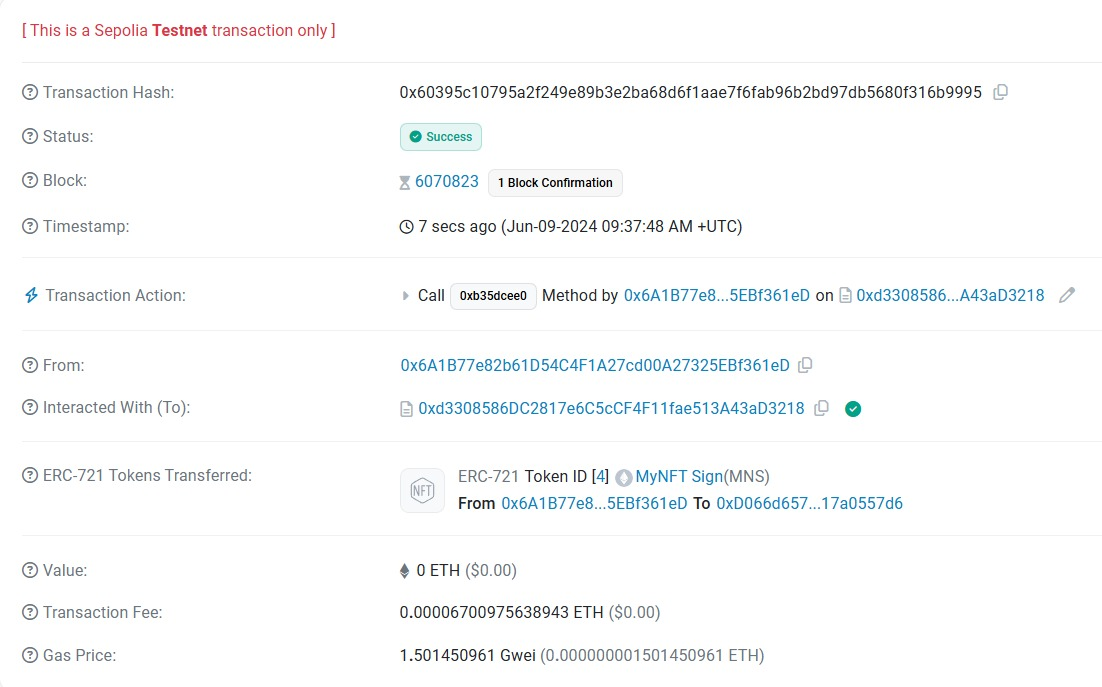
\includegraphics[scale=0.20]{gambar/detail_pada_etherscan.jpeg}}
    % Caption for the image
    \caption{Details on Etherscan}
    % Reference label for the image
    \label{fig:details_etherscan}
    \end{figure}

    \item On Etherscan, details of the NFT can also be checked for ownership. As seen from the image \ref{fig:detail_nft_etherscan}, the owner of NFT \#4 is the address of user A on the Sepolia Ethereum Testnet, then in the image below, after successfully performing the bridge transfer, the ownership changes to user B on the BNB Chain Testnet.

    \begin{figure} [H] \centering
    % Name of the image file
    \frame{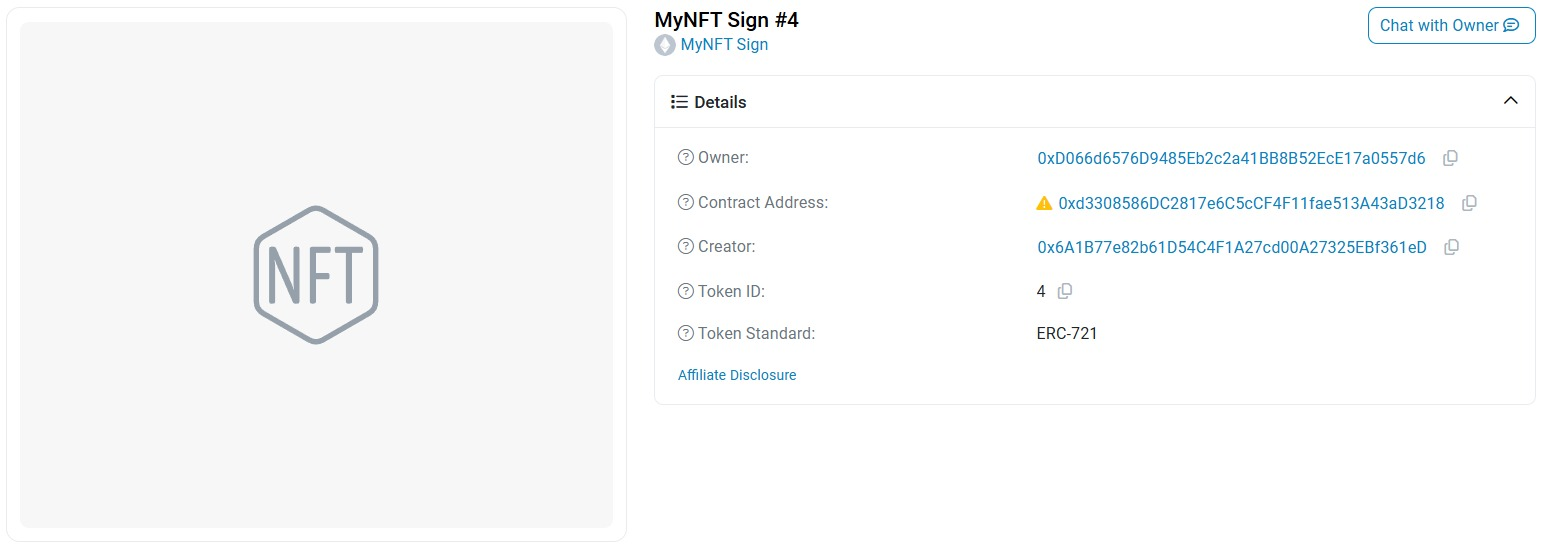
\includegraphics[scale=0.165]{gambar/nft_detail_etherscan2.jpeg}}
    % Caption for the image
    \caption{NFT details on Etherscan after bridge transfer}
    % Reference label for the image
    \label{fig:nft_bridge_transfer}
    \end{figure}

    \item On the OpenSea platform, the NFT sent to the address of user B can also be seen.

    \begin{figure} [H] \centering
    % Name of the image file
    \frame{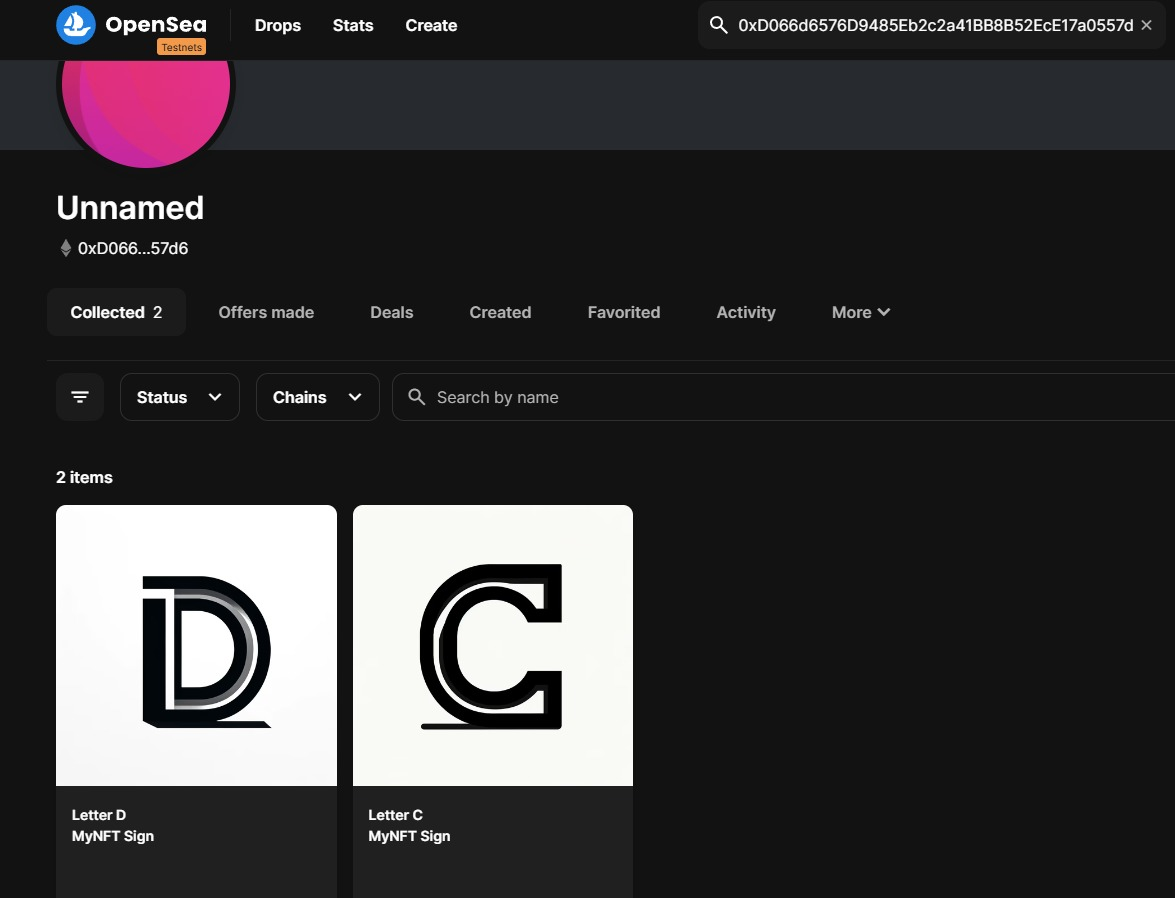
\includegraphics[scale=0.15]{gambar/nft_pada_opensea_2.jpeg}}
    % Caption for the image
    \caption{NFT on OpenSea at the address of B}
    % Reference label for the image
    \label{fig:opensea2}
    \end{figure}
    
\end{itemize}

  % Ubah judul dan label berikut sesuai dengan yang diinginkan.
\section{Conclusion}
\label{sec:kesimpulan}

% Ubah paragraf-paragraf pada bagian ini sesuai dengan yang diinginkan.
In this research, we have explored and implemented the concept of blockchain-based NFT interoperability using smart contracts within the context of the Metaverse and Web3.0. This study has successfully demonstrated the potential and effectiveness of blockchain technology, particularly Ethereum, in supporting the creation and management of NFTs that can operate across various tokens.
% \subsection{Conclusions from this research are}
% \begin{itemize}
%     \item Smart Contract Implementation: The designed smart contracts have successfully facilitated the creation, transactions, and verification of NFTs securely and efficiently. By using the ERC-721 standard, we have implemented unique NFTs that can be traced to their origin, which is essential in the Metaverse and Web3.0 ecosystems.
%     \item The developed NFTs show high interoperability across various Metaverse platforms. This was achieved through the use of consistent protocols and APIs, allowing the NFTs to be used in various applications and games within the Web3.0 ecosystem without substantial modifications.

% % \subsection{Recommendations for further development}
% % To enhance the interoperability and efficiency of NFT usage in the Metaverse, it is recommended that future research focus on developing more universal protocols for cross-chain integration. Additionally, further research is needed to refine security mechanisms that can protect user privacy while maintaining the transparency and reliability of the blockchain system.
% \end{itemize} 



  % Menampilkan daftar pustaka dengan format IEEE
  \bibliographystyle{IEEEtranN}
  \bibliography{pustaka/pustaka.bib}

  % Menyeimbangkan bagian akhir di kedua kolom
  \balance

\end{document}